\documentclass{article}
\usepackage[papersize={6.95in,3.55in},margin=9pt]{geometry}
% Shared visual grammar for FIGURE_FREEZE_V1.
% One blue family + grayscale. Meaning also encoded by shape/border.
\usepackage[T1]{fontenc}
\usepackage{lmodern}
\usepackage{amsmath,amssymb}
\usepackage{tikz}
\usetikzlibrary{arrows.meta,positioning,fit,calc,matrix}

\definecolor{ink}{HTML}{22272B}
\definecolor{muted}{HTML}{5C6770}
\definecolor{rule}{HTML}{B7C0C7}
\definecolor{band}{HTML}{F3F5F7}
\definecolor{accent}{HTML}{2E5A88}
\definecolor{accentfill}{HTML}{E7F0F6}

\tikzset{
  arr/.style={-{Latex[length=2.1mm,width=1.6mm]}, line width=0.6pt, draw=ink},
  arrd/.style={-{Latex[length=2.1mm,width=1.6mm]}, densely dashed, line width=0.6pt, draw=muted},
  figbase/.style={
    font=\small\selectfont,
    color=ink,
    line cap=round,
    line join=round,
  },
  box/.style={
    draw=ink, line width=0.55pt,
    rounded corners=1.4pt,
    inner sep=3.6pt,
    align=center,
    text=ink,
  },
  boxplain/.style={box, fill=white},
  boxband/.style={box, fill=band, draw=rule},
  boxaccent/.style={box, fill=accentfill, draw=accent, line width=0.7pt},
  untrusted/.style={box, densely dashed, draw=muted, fill=white},
  badge/.style={
    font=\footnotesize\selectfont,
    inner sep=2.2pt,
    align=center,
    draw, line width=0.6pt,
    rounded corners=1.1pt,
  },
  badgeexact/.style={badge, fill=accentfill, draw=accent},
  badgesubst/.style={badge, fill=white, draw=accent, densely dashed},
  badgerule/.style={badge, fill=white, draw=ink, double, double distance=1.05pt},
  badgeunk/.style={badge, fill=white, draw=muted, dotted},
  badgerefuse/.style={badge, fill=white, draw=ink, dashed},
  lab/.style={font=\footnotesize\selectfont, text=muted, align=center, inner sep=1pt},
  head/.style={font=\normalsize\bfseries\selectfont, text=accent, align=center},
  axislab/.style={font=\footnotesize\selectfont, text=ink},
}

\pagestyle{empty}
\setlength{\parindent}{0pt}
\begin{document}
\centering
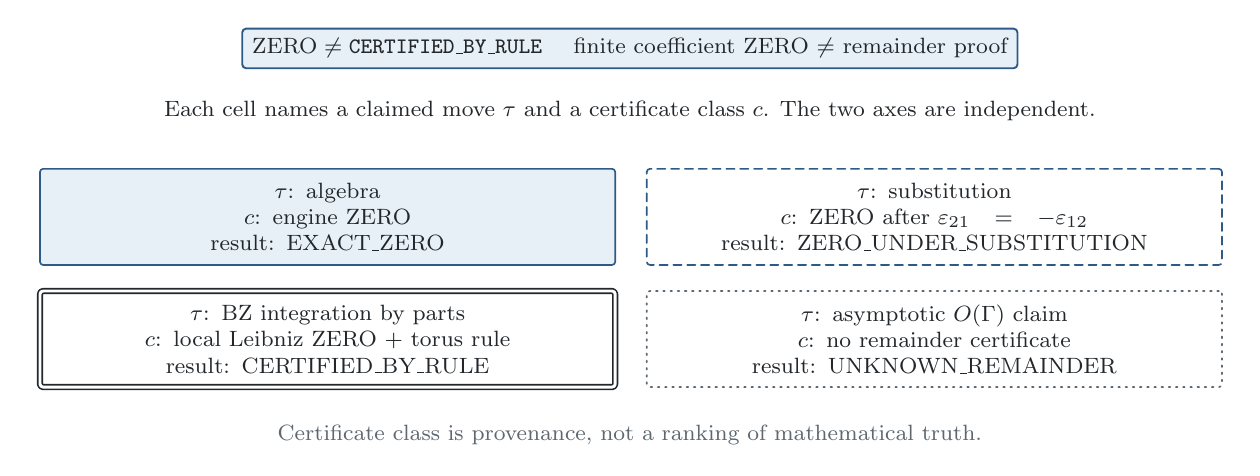
\begin{tikzpicture}[figbase]
  \node[boxaccent, font=\footnotesize\selectfont] (ban)
    {$\mathrm{ZERO}\neq\texttt{CERTIFIED\_BY\_RULE}$
     \quad finite coefficient ZERO $\neq$ remainder proof};
  \node[axislab, below=8pt of ban] (sub)
    {Each cell names a claimed move $\tau$ and a certificate class $c$. The two axes are independent.};

  \matrix (m) [
    below=10pt of sub,
    matrix of nodes,
    row sep=8pt,
    column sep=10pt,
    nodes={
      anchor=center,
      align=left,
      font=\footnotesize\selectfont,
      text width=7.15cm,
      minimum height=1.22cm,
      inner sep=5pt,
    },
  ] {
    |[badgeexact]| {$\tau$: algebra\\$c$: engine ZERO\\result: EXACT\_ZERO}
    & |[badgesubst]| {$\tau$: substitution\\$c$: ZERO after $\varepsilon_{21}=-\varepsilon_{12}$\\result: ZERO\_UNDER\_SUBSTITUTION} \\
    |[badgerule]| {$\tau$: BZ integration by parts\\$c$: local Leibniz ZERO $+$ torus rule\\result: CERTIFIED\_BY\_RULE}
    & |[badgeunk]| {$\tau$: asymptotic $O(\Gamma)$ claim\\$c$: no remainder certificate\\result: UNKNOWN\_REMAINDER} \\
  };

  \node[lab, below=8pt of m]
    {Certificate class is provenance, not a ranking of mathematical truth.};
\end{tikzpicture}
\end{document}
